Les diagrammes de séquences systèmes réalisés durant l'étape
de conception du bureau distribué sont représentés dans cette 
partie. Il y en a un par cas d'utilisation. 
Ils sont tous représentatifs de la phase de conception du projet
mais ils pourront etre corrigés si les technologies utilisées
varient d'ici l'étape de développement.

\section{Se connecter au bureau distribué}

Ce premier diagramme de séquence système relate le cas d'utilisation
1, qui consiste en la connexion d'un utilisateur au bureau distribué.

\begin{figure}[h!]
	\centering
	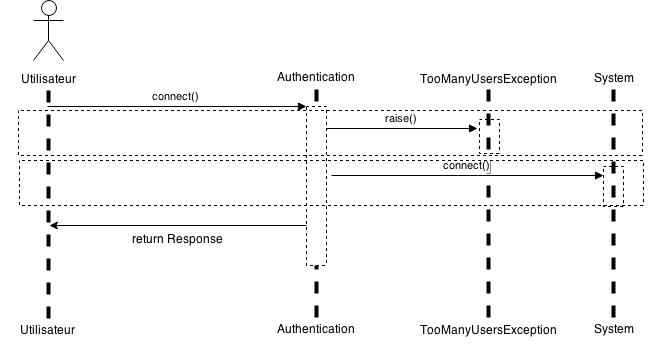
\includegraphics[scale=0.4]{diagrammes/DSS1.jpg}
	\caption{Diagramme de Séquence Système, cas 1}
\end{figure}

\section{Ouvrir une fenetre}

Ce second diagramme de séquence système relate le cas d'utilisation
2, qui consiste en l`ouverture par un utilisateur d'une nouvelle 
fenetre (widget).

\begin{figure}[h!]
	\centering
	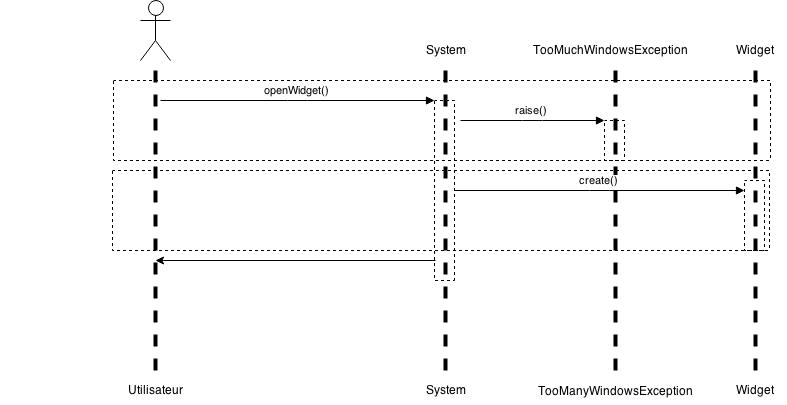
\includegraphics[scale=0.4]{diagrammes/DSS2.jpg}
	\caption{Diagramme de Séquence Système, cas 2}
\end{figure}

\section{Saisir une opération}

Ce troisième diagramme de séquence système relate le cas d'utilisation
3, qui consiste en la saisie d'une opération par l'utilisateur dans la 
calculatrice.

\begin{figure}[h!]
	\centering
	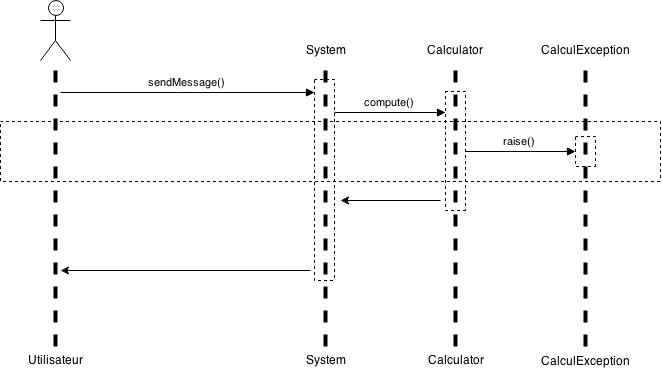
\includegraphics[scale=0.4]{diagrammes/DSS3.jpg}
	\caption{Diagramme de Séquence Système, cas 3}
\end{figure}

\section{Regarder des photos}

Ce quatrième diagramme de séquence système relate le cas d'utilisation
4, qui consiste à regarder des photos dans le widget galerie.

\begin{figure}[h!]
	\centering
	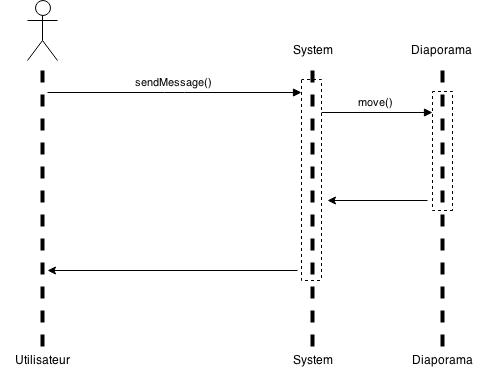
\includegraphics[scale=0.4]{diagrammes/DSS4.jpg}
	\caption{Diagramme de Séquence Système, cas 4}
\end{figure}

\section{Quitter le bureau virtuel}

Enfin, le dernier diagramme de séquence système relate le cas d'utilisation
5, qui consiste à se déconnecter du bureau virtuel.

\begin{figure}[h!]
	\centering
	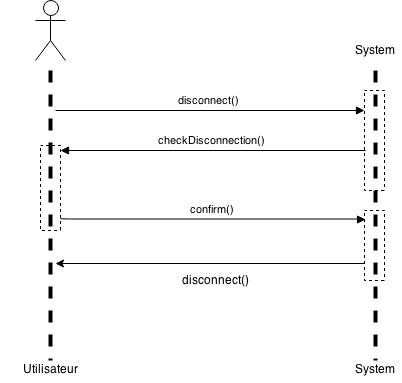
\includegraphics[scale=0.4]{diagrammes/DSS5.jpg}
	\caption{Diagramme de Séquence Système, cas 5}
\end{figure}
